\documentclass[UTF8]{ctexart}

\usepackage{amsmath}
\usepackage{listings}
\usepackage{amsfonts}
\usepackage{graphicx}
\usepackage{hyperref}
\usepackage{algorithm}
\usepackage{algpseudocode}
\usepackage{geometry}



\geometry{
    a4paper, % 页面纸张大小
    left=2.8cm, % 左边距
    right=2.8cm, % 右边距
    top=2cm, % 上边距
    bottom=2cm, % 下边距
    includehead, % 包括页眉
    includefoot % 包括页脚
}

\title{流动与配对-\\图论中网络最大流问题与最大匹配问题探讨}
\author{曹奕伦 22300240008}
\date{\today}

\begin{document}


\maketitle


\section{论文摘要}

论文主要探讨了网络最大流问题中的基础定理与实际应用算法,包括Max-flow-Min-cut定理\cite{enwiki:1192320700}、Ford-Fulkerson算法\cite{ford1956maximal}、Edmonds-Karp算法\cite{edmonds1972theoretical}、Dinic算法\cite{dinitz1970algorithm},以及最大匹配中的基础定理与实际应用算法,包括Berge引理\cite{berge1957two}、Hall定理\cite{hall1987representatives}、Tutte定理\cite{tutte1950factorization}、Tutte-Berge公式\cite{berge1958couplage}、Konig定理\cite{kHonig1931grafok}、Hopcroft-Karp算法\cite{hopcroft1973n}、Hungarian算法\cite{munkres1957algorithms}、Bloosom算法\cite{edmonds1965paths}等内容。


\section{背景介绍}


\subsection{最大流问题}

网络流是图论中一个重要的概念,它在模拟各种实际情况中都有广泛的应用。一个网络流问题可以用图来表示,其中节点代表各种资源或位置,边代表资源之间的流动路径或连接。

在网络流问题中,每条边都有一个容量限制,表示该路径能够承载的最大流量。流量可以在图中的路径上流动,但不能超过每条路径的容量限制。这一概念在模拟实际世界中的管道、道路、数据传输等方面有着广泛的应用。

最大流问题是网络流问题中的一个重要分支,它着重于寻找从一个特定起点到一个特定终点的最大流量路径。这个问题通常涉及如何在网络中找到一条路径,使得其流经的边的总流量最大化,同时满足每条路径的容量限制。

解决最大流问题的算法和技术对于优化网络资源分配、流量控制、通信网络以及运输规划等领域都具有重要意义。通过寻找最大流量路径,我们能够最大化资源的利用,提高系统的效率和性能。

在解决最大流问题的过程中,有许多经典的算法和技术被提出和优化,其中包括Ford-Fulkerson算法\cite{ford1956maximal}、Edmonds-Karp算法\cite{edmonds1972theoretical}、Dinic算法\cite{dinitz1970algorithm}等。这些算法在寻找网络中的最大流路径方面都发挥着重要作用。


\subsection{最大匹配问题}

在图论中,匹配是一种重要的概念,用于描述图中节点之间的配对关系。一个匹配是图中边的集合,其中任意两条边没有共同的顶点。在匹配中,每个顶点最多只能属于一条边。这个概念在实际应用中常用于模拟配对问题,如任务分配、婚姻问题等。

其中最大匹配问题包括了二分图最大基数匹配问题、二分图最大权重匹配问题、一般图最大基数匹配问题和一般图最大权重匹配问题等。其中二分图最大基数匹配问题是最大匹配问题中的一个基础问题,其他问题都可以视作二分图最大基数匹配问题的衍生变种。

解决最大匹配问题对于任务分配、资源优化、稳定婚姻问题等领域有着广泛的应用。通过寻找图中的最大匹配,我们能够有效地优化资源分配,实现任务的最优解决方案,或者找到稳定的配对关系。

在解决最大匹配问题的过程中,有许多经典的算法和技术被提出和优化,其中包括Hopcroft-Karp算法\cite{hopcroft1973n}、Hungarian算法\cite{munkres1957algorithms}、Bloosom算法\cite{edmonds1965paths}等。这些算法在寻找图中的最大匹配方面都发挥着重要作用。



\section{论文内容}


\subsection{最大流问题}

\subsubsection{基础定义与定理}

\begin{enumerate}
      \item
            \textbf{网络的定义:}

            设连通无自环的带权有向图G,其中有两个不同的顶点s和t,其中s为源点(source),t为汇点(sink),且每条边的权值都是非负实数,则称该有向图为网络,记为N(V,E,C),其中C为网络的容量函数


      \item
            \textbf{流量的定义: }

            设$N(V,E,C)$为网络,则流量$f$是$N$上的一个实函数。

            对于任意一条边$e=(u,v)$,有$f(e)\le C(e)$

            对于中间点k,有$\sum f(j,k)=\sum f(k,i)$,

            即 k入流量=k出流量,k负责传递流量

            对于源点s,有$\sum f(j,s)+V_f=\sum f(s,i)$,

            即 s入流量+流=s出流量,s能够产生流量

            对于汇点t,有$\sum f(j,t)-V_f=\sum f(t,i)$,

            即 t入流量-流=t出流量,t能够消耗流量

            其中$V_f$称为f的流量,如果没有其他f'使得$V_{f'}>V_f$,则称f为最大流

      \item
            \textbf{饱和的定义: }


            若$f(i,j)=C(i,j)$,则称弧e=(i,j)为饱和的

            若$f(i,j)<C(i,j)$,则称弧e=(i,j)为未饱和的

      \item
            \textbf{割的定义: }

            设N(V,E,C)是网络,s为其源点,t为其汇点

            若V被分割为两个不相交的子集$A,A^C$,使得$s\in A,t\in A^C$,

            那么称 从$A$到$A^C$的弧集 为割,记为$(A,A^C)$

            割$(A,A^C)$的容量为其所有弧的容量之和,即$C(A,A^C)=\sum_{i\in A,j\in A^C}C_{ij}$

            若N中不存在其他割$(A',A'^C)$,使得$C(A',A'^C)<C(A,A^C)$,则称$(A,A^C)$为最小割


      \item
            \textbf{引理: }

            对于任意网络N(V,E,C),设f是N上的任一可行流,$(A,A^C)$是N的任一割,则有$V_f\le C(A,A^C)$

            证明:由于$s\in A$,则$A$能够产生流量,

            即$\sum f(A,A^C)=\sum f(A^C,A)+V_f$

            因为$\sum f(A^C,A)$是个非负值,所以$\sum f(A^C,A)+V_f\ge V_f$

            故$V_f\le\sum f(A,A^C)\le C(A,A^C)$,得证

      \item
            \textbf{最大流最小割定理(Max-flow Min-cut theorem):}\cite{enwiki:1192320700}

            在任意网络中,从s到t的最大流等于网络的最小割

            定义残差容量函数$c_f:V\times V\to R^+$,使得

            1. 如果$(i,j)\in E$,那么$c_f(i,j)=C(i,j)-f(i,j)$

            2. 如果$(j,i)\in E$,那么$c_f(i,j)=f(j,i)$

            用构造法证明:给定最大流f,现构造增广路点集A为

            1. $s\in A$

            2. $if\ (i \in A) \land (c_f(i,j) > 0) \to j\in A$

            如果$t\in A$,那么就存在一条从s到t的增广路,使得最大流f的流量增加,得出矛盾

            故$t\notin A$,于是得到分离s和t的割$(A,A^C)$

            由增广路的构造过程可知,对于任意$k\in A,k'\in A^C$,

            要么有$f(k,k')=C(k,k')$,要么有$f(k,k')=0$

            也就是说,对于割$(A,A^C)$,

            1. 所有正向弧的流量都是饱和的

            2. 所有反向弧的流量都为0

            即$\sum f(A,A^C)=\sum C(A,A^C)$,$\sum f(A^C,A)=0$

            因为引理已证得$\sum f(A,A^C)=\sum f(A^C,A)+V_f$

            故有$\sum C(A,A^C)=V_f$,得证
\end{enumerate}

\vspace{10cm}

\subsubsection{算法实现与时间复杂度分析}

\begin{enumerate}
      \item

            \textbf{Ford-Fulkerson算法 }\cite{ford1956maximal}

            \begin{algorithm}
                  \caption{Ford-Fulkerson Algorithm}
                  \begin{algorithmic}[1]
                        \Procedure{find maximum flow}{$G$}
                        \State \textbf{Input:} Network G=(V,E,C)
                        \State \textbf{Output:} Maximum flow of Network G
                        \State
                        \For{each edge(u,v)$\in$G,E}
                        \State f(u,v)=0
                        \EndFor
                        \State
                        \While{exists a path $p$ from $s$ to $t$ in residual network $G_f$}
                        \State $c_f(p)=\min\{c_f(p):(u,v)\in p\}$
                        \For{each edge$(u,v)\in p$}
                        \If{$(u,v)\in E$}
                        \State $f(u,v)=f(u,v)+c_f(p)$
                        \ElsIf{$(v,u)\in E$}
                        \State $f(v,u)=f(v,u)-c_f(p)$
                        \EndIf
                        \EndFor
                        \EndWhile
                        \State \textbf{return} $f$
                        \EndProcedure
                  \end{algorithmic}
            \end{algorithm}


            \vspace{0.5cm}

            当网络的容量为整数时,Ford-Fulkerson算法的时间复杂度为$O(Ef)$

            其中E为网络中的边数,f为最大流的流量

            这是因为在每次迭代中,算法需要在$O(E)$时间内找到增广路

            而对于每次迭代,流量至少增加1,最多增加$f$,故最多需要$O(f)$次迭代



            \vspace{3cm}

      \item
            \textbf{Edmonds-Karp算法}\cite{edmonds1972theoretical}

            将Ford-Fulkerson算法中的搜索增广路径过程改为BFS,即可得到Edmonds-Karp算法

            现欲证明Edmonds-Karp算法的时间复杂度为$O(VE^2)$

            \vspace{1.2cm}


            \paragraph{- 引理}
            对于任意顶点$v\in V-\{s,t\}$,从s到达v所需的最短增广路径距离$\delta_f(s,v)$随着迭代次数增加而单调递增

            用反证法证明:假设存在一个增广操作,使得$\delta_f(s,v)$减小为$\delta_{f'}(s,v)$,

            并且v是所有因增广操作递减的顶点中,$\delta_{f'}(s,v)$最小的顶点

            不妨假设在残差网络$G_{f'}$中,从s到v的最短路径$p=s\sim u\to v$

            所以$(u,v)\in E_{f'}$,并且$\delta_{f'}(s,v)=\delta_{f'}(s,u)+1$

            因为v是$\delta_{f'}(s,v)$最小的顶点,而u不是,所以$\delta_{f'}(s,u)\ge\delta_f(s,u)$

            如果有$(u,v)\in E_f$,那么
            $$
                  \begin{aligned}
                        \delta_f(s,v) & \le\delta_f(s,u)+1    \\
                                      & \le\delta_{f'}(s,u)+1 \\
                                      & =\delta_{f'}(s,v)
                  \end{aligned}
            $$
            这与之前的假设$\delta_{f'}(s,v)<\delta_f(s,v)$矛盾,所以$(u,v)\notin E_f$

            所以要使得$(u,v)\notin E_f$,而$(u,v)\in E_{f'}$,那么f就要有从v到u的最短路径$p=s\sim v\to u$,那么
            $$
                  \begin{aligned}
                        \delta_f(s,v) & \le\delta_f(s,u)-1    \\
                                      & \le\delta_{f'}(s,u)-1 \\
                                      & =\delta_{f'}(s,v)-2
                  \end{aligned}
            $$
            这又与之前的假设$\delta_{f'}(s,v)<\delta_f(s,v)$矛盾,所以不存在这样的顶点v

            \vspace{1cm}

            \paragraph{- 定理}
            Edmonds-Karp算法的时间复杂度为$O(VE^2)$

            如果在残差网络$G_f$中,增广路p的最大容量$c_f(p)=c_f(u,v)$,那么将(u,v)称为这条增广路p的关键边

            如果(u,v)是首次成为关键边,那么有$\delta_f(s,v)=\delta_f(s,u)+1$

            因为这时候(u,v)已经饱和,所以如果还想成为关键边,那么就需要成为抵消操作,即$(v,u)\in E_{f'}$

            所以有$\delta_{f'}(s,u)=\delta_{f'}(s,v)+1$

            由引理可知,对于顶点v有$\delta_{f'}(s,v)\ge\delta_f(s,v)$,所以
            $$
                  \begin{aligned}
                        \delta_{f'}(s,u) & =\delta_f(s,v)+1      \\
                                         & \ge\delta_{f'}(s,v)+1 \\
                                         & =\delta_{f'}(s,u)+2
                  \end{aligned}
            $$
            故每次操作最多会使顶点u的距离增加2,
            \vspace{10cm}

            因为顶点u到v的距离最多为$|V|-2$,

            所以(u,v)最多需要$(|V|-2)/2=|V|/2-1$次操作迭代

            而图G中总共有$|E|$条边,

            所以对于所有边来说,最多需要$O(VE)$次操作迭代

            因为每次操作的时间复杂度为$O(E)$,所以总的时间复杂度为$O(VE^2)$


            \vspace{2cm}

      \item

            \textbf{Dinic算法}\cite{dinitz1970algorithm}

            将Ford-Fulkerson算法中的搜索增广路径过程改为启发式搜索,即可得到Dinic算法

            1. 将每条边的流量初始化为0,即$\forall e\in E,f(e)=0$

            2. 从残差图$G_f$中构造 层级残差图$G_L$,使得对于残差容量$c_f(u,v)>0$的边(u,v),有$L(v)=L(u)+1$

            3. 在 层级残差图$G_L$中,从s到t搜索一条 层级增广路p,使得$\forall (u,v)\in p,L(v)=L(u)+1$

            4. 将层级增广路p累加至流f中,并不断重复步骤2和步骤3,直到不存在层级增广路为止

            \vspace{1cm}


            \paragraph{- 定理 }

            Dinic算法的时间复杂度为$O(V^2E)$

            由于在每次迭代中,层级流的层数最多将增加1,而层级流的层数最多为$|V|-1$,所以迭代次数为$O(V)$,而对于每次迭代有:

            1. 使用BFS构造层级残差图$G_L$的时间复杂度为$O(E)$

            2. 使用DFS搜索层级增广路p的时间复杂度为$O(VE)$

            所以每次迭代的时间复杂度为$O(E+VE)=O(VE)$,故总时间复杂度为$O(V^2E)$,得证


\end{enumerate}

\vspace{1cm}


\subsection{最大匹配问题}

\subsubsection{基础定义与定理}


\begin{enumerate}
      \item

            \textbf{匹配的定义(Matching or Independent-edge-set)}

            设图G(V,E)是一个无向图,有$M\subseteq E$

            如果M中的任意两条边都没有公共点,则称M为G的一个匹配



      \item

            \textbf{盖点的定义(Matched or Saturated Vertex) }

            设M是二分图G的一个匹配,将M中的边所关联到的顶点称为盖点



      \item

            \textbf{极大匹配的定义(Maximal matching) }

            设图G的一个匹配为M,如果M不是其他任何匹配的真子图,则称M为极大匹配



      \item

            \textbf{最大匹配的定义(Maximum matching or Maximum-cardinality matching) }

            设图G的一个匹配为M,如果M的边数大于其他任何匹配的边数,则称M为最大匹配

            将最大匹配的边数称为图G的匹配数,记为$\nu(G)$





      \item
            \textbf{完美匹配的定义(Perfect matching or Complete matching) }

            设图G的一个匹配为M,如果M的盖点数等于图G的顶点数,则称M为完美匹配

            完美匹配同时也是最小边覆盖

            完美匹配需要顶点数为偶数

            完美匹配同时也是最大匹配


      \item


            \textbf{准完美匹配的定义(Near-perfect matching) }

            设图G的一个匹配为M,如果M的盖点数只比图G的顶点数少1,则称M为准完美匹配

            准完美匹配需要顶点数为奇数

            准完美匹配同时也是最大匹配


      \item


            \textbf{交错路和增广路的定义(Alternating path and Augmenting path)}

            若一条路由未盖点开始,路上属于匹配M的边和不属于匹配M的边交错出现,则称该路为交错路

            如果路p是一条起始点和结束点都是未盖点的交错路,则称路p为增广路

            \vspace{1cm}

      \item

            \textbf{引理}

            将增广路p进行匹配边与非匹配边的对换,得到$M\oplus p$

            则$M\oplus p$也是关于图G的匹配,且比M多了一条匹配边

            证明:由于增广路的两端都是未盖点,所以不会影响到其他边的匹配

            而将增广路进行对换之后仍然满足匹配,且多了一条匹配边,得证

            \vspace{1cm}

      \item

            \textbf{引理}

            对于图G,以及图G的两个匹配M和M',令$G'=M\oplus M'$,则G'由以下三种组成:

            1. 孤立点

            2. 具有M和M'交错边的偶回路

            3. 具有M和M'交错边的交错路

            \vspace{3cm}

            证明: G'中每个顶点最多与2条边相关联,

            其中一条来自M,另一条来自M'

            因此,图G'只能由由孤立顶点、回路或交替路径组成

            而对于回路,它必须具有相等数量来自M和M'的交错边,因此其长度必须为偶数,即其为具有M和M'交错边的偶回路,得证


            \vspace{2cm}


      \item


            \textbf{Berge定理 (Berge's theorem)}\cite{berge1957two}

            匹配M为图G的最大匹配,当且仅当图G中不存在关于M的增广路

            逆否命题:匹配M不是图G的最大匹配,当且仅当图G中存在关于M的增广路

            $\impliedby$:证明:假设图G中存在关于M的增广路

            那么将增广路进行对换,就能得到$|M\oplus p|>|M|$,故M不是最大匹配,得证

            $\implies$:证明:假设M不是最大匹配,那么存在一个最大匹配$M'$,使得$|M'|>|M|$,

            作$D=M'\oplus M$,由引理知,$D$的各连通分支皆为关于M和M'的偶回路或者交错路

            由于$|M'|>|M|$,那么在$D$中,就会存在某个连通分支,

            使得其中属于M'的边数大于属于M的边数

            那么这个连通分支就是一条以M'的边作为首尾的交错路p,所以是关于M的增广路,得证

            \vspace{1cm}

      \item


            \textbf{霍尔婚配定理(Hall's Marriage Theorem)}\cite{hall1987representatives}

            对于二分图$G(X,Y)$,存在X-完美匹配,当且仅当对于$X$的任意子集A,以及与A邻接的点集N(A),都有$|N(A)|\ge|A|$

            $\implies$:因为存在X-完美匹配,所以X的任意子集A也都存在完美匹配,故$|N(A)|\ge|A|$

            $\impliedby$:要证明:若对于任何子集$A\subseteq X$,都有$|N(A)|\ge|A|$,那么存在X-完美匹配

            逆否命题:如果不存在X-完美匹配,那么就会存在子集$A\subseteq X$,使得$|N(A)|<|A|$


            由于不存在X-完美匹配,即最大匹配M不是X-完美匹配,所以X中存在未盖点$u\in X$,以u为根节点构造交错树T

            记X的子集A为交错树T在X中的点集,记Y的子集B为交错树T在Y中的点集,即$A=X\cap T,B=Y\cap T$

            由于M是最大匹配,所以子集B中所有顶点都是盖点,否则能构造出关于M的增广路,得到更大的匹配

            因为匹配边在交错树中的方向是从右到左的,所以子集A中的盖点数=子集B中的盖点数

            又因为X中还有个未盖点$u\in X$,所以$|A|=|B|+1>|B|$,即$|N(A)|<|A|$,得证




      \item

            \textbf{塔特定理(Tutte Theorem)}\cite{tutte1950factorization}

            Tutte定理是Hall定理的推广

            \vspace{0.5cm}

            \textbf{奇组件的定义(Odd component)}

            如果一个连通分支的顶点数为奇数,那么称这个连通分支为奇组件

            \vspace{0.5cm}

            对于任意图$G(V,E)$,存在完美匹配,

            \textbf{当且仅当} 对于$V$的任意子集U,以及与U邻接的奇组件odd(G-U),都有$|U|\ge|odd(G-U)|$

            $\implies$:因为存在完美匹配,所以每个奇组件至少有一个顶点需要与U中的顶点匹配,

            所以有$|U|\ge|odd(G-U)|$,充分性得证

            $\impliedby$:要证明:若对于任何子集$U\subseteq V$,都有$|U|\ge|odd(G-U)|$,那么存在完美匹配

            逆否命题:如果不存在完美匹配,那么就会存在子集$U\subseteq V$,使得$|U|<|odd(G-U)|$

            对于子集$U\subseteq V$,如果能够使得$|U|=|odd(G-U)|$,那么称子集U为关键子集

            现取出图G的最大关键子集记为W,则W具有如下几个性质:

            \vspace{0.5cm}

            1. 图G-W中不存在偶组件,否则可以从偶组件中取出v,使得$W'=W\cup\{v\}$,并且$|W'|>|W|$,与W是最大关键子集矛盾

            2. 对于图G-W中的任意奇组件C,从奇组件C中取出v,可以使得$C-\{v\}$存在完美匹配

            \vspace{0.5cm}

            所以可以将分支集合族$odd(G-U)$看作是二分图中的点集X,将最大关键子集W看作是二分图中的点集Y,因为不存在完美匹配,所以根据Hall定理可知,存在子集$A\subseteq X=odd(G-U)$,使得$|N(A)|<|A|$

            即存在子集$U=N(A)=N(odd(G-U))\subseteq W\subseteq V$,使得$|U|<|odd(G-U)|$,得证


            \vspace{1cm}

      \item

            \textbf{Tutte-Berge公式}\cite{berge1958couplage}

            从直观上来说就是,由于每个奇组件都会自带一个未匹配点,所以有$odd(G-U)$,而这个未匹配点可以被$U$中的未匹配点所抵消,即$odd(G-U)-|U|$

            任意图G(V,E)的最多未匹配点为$\max_{U\subseteq V}(odd(G-U)-|U|)$

            或者说:任意图G(V,E)最大匹配数为 $\frac{1}{2}\min_{U\subseteq V}(|V|-odd(G-V)+|U|)$


            \vspace{3cm}


      \item

            \textbf{Konig定理}\cite{kHonig1931grafok}

            在二分图$G(X,Y)$中,有最大匹配数等于最小点覆盖数


            \vspace{0.5cm}


            \textbf{- 使用最大流最小割构造最小点覆盖来证明:}

            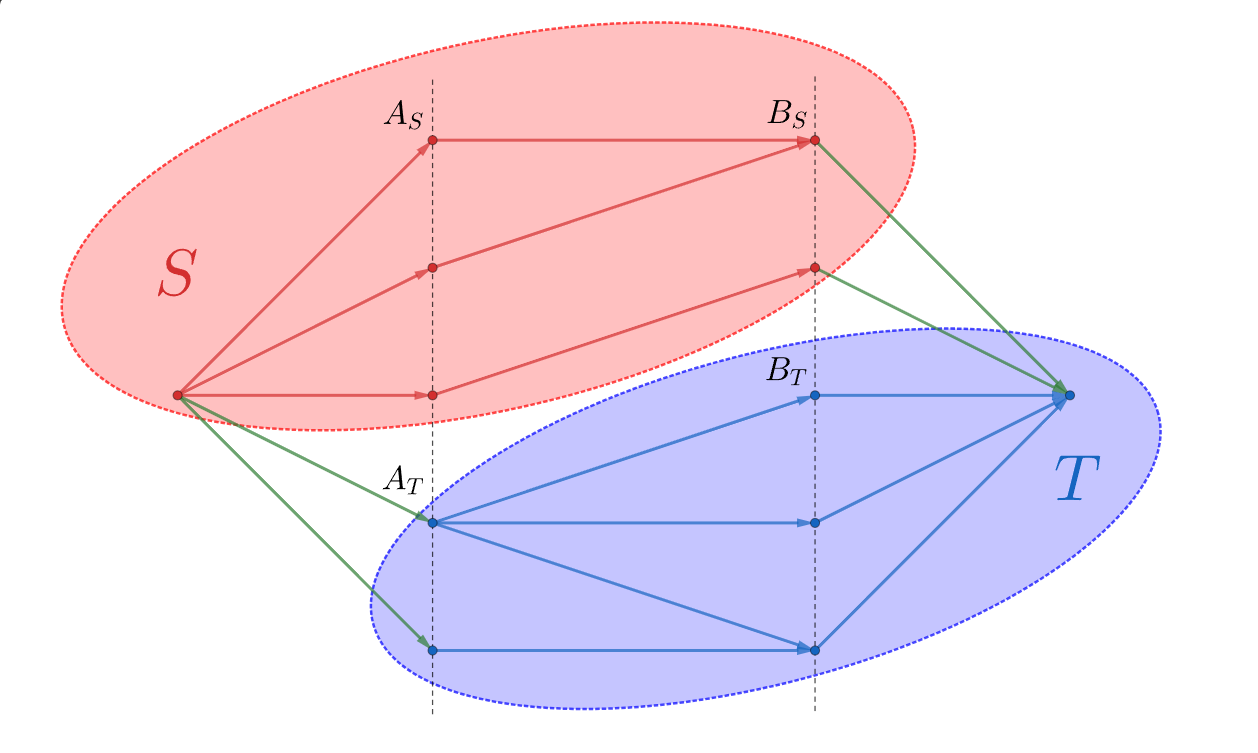
\includegraphics[width=0.5\textwidth]{img/Minimum_cut_in_a_bipartite_graph.png}

            已知二分图G(A,B),并且有最大匹配M,现构造最小点覆盖

            构造流网络$G'_\infty$,其中从源点s流向A的容量为1,

            从A流向B的容量为$\infty$,从B流向汇点t的容量为1

            由最大匹配和最大流的定义可知,此时$|M|=V_f$,故可以运用最大流最小割定理

            取出最小割$(S,T)$,且$A=A_S\cup A_T,B=B_S\cup B_T$,

            则最小割只包含 从s到$A_T$的边 和 从$B_S$到t的边,

            因为所有 从$A_S$到$B_T$的 和 从$A_T$到$B_S$的 无穷边都会导致割的流量为无穷大

            所以最小割的大小为$|A_S|+|B_T|$,并且$A_T\cup B_S$是点覆盖

            即点覆盖的大小为$|A_S|+|B_T|=|M|$,所以这是最小点覆盖,得证

            \vspace{3cm}


            \textbf{- 使用交错树构造最小点覆盖来证明:}

            已知二分图G(X,Y),并且有最大匹配M,现构造最小点覆盖

            考虑以下构造:取左侧X的未匹配结点作为根节点,构造多棵交错树

            然后再将所有交错树上的所有结点都打上标记,记为点集Z

            最后再构造集合K为:X未打标记的结点+Y打了标记的结点

            即 $K=(X-Z)\cup(Y\cap Z)$

            现欲证明集合K是一个点覆盖,且$|K|=|M|$

            \vspace{2.5cm}

            首先证明:集合K是一个点覆盖,即所有边都要么左侧未打标记,要么右侧打了标记

            逆否命题:不存在这样的边,其左侧打了标记,并且右侧没打标记

            \vspace{0.3cm}

            1. 假设存在 左侧打了标记 and 右侧没打标记 的匹配边,因为匹配边在交错树中的方向是从右到左的,所以如果右侧没标记,那么左侧也不应该有标记,得出矛盾

            2. 假设存在 左侧打了标记 and 右侧没打标记 的非匹配边,因为非匹配边在交错树中的方向是从左到右的,所以如果左侧有标记,那么右侧也应该有标记,得出矛盾

            \vspace{0.8cm}

            因为K是点覆盖,由引理可知$|K|\ge|M|$,

            所以要证明K是最小点覆盖,还需要证明$|K|\le|M|$,即K中的所有点都会被匹配边覆盖

            \vspace{0.3cm}

            1. 对于左侧X未打标记的结点,其肯定不能是未盖点,否则会作为交错树根结点

            2. 对于右侧Y打了标记的结点,其肯定不能是未盖点,否则会出现增广路

            \vspace{0.2cm}

            综上所述,集合K是一个点覆盖,且$|K|=|M|$,所以K是最小点覆盖,得证

            \vspace{1cm}



            \textbf{- 使用Hall定理构造最大匹配来证明:}

            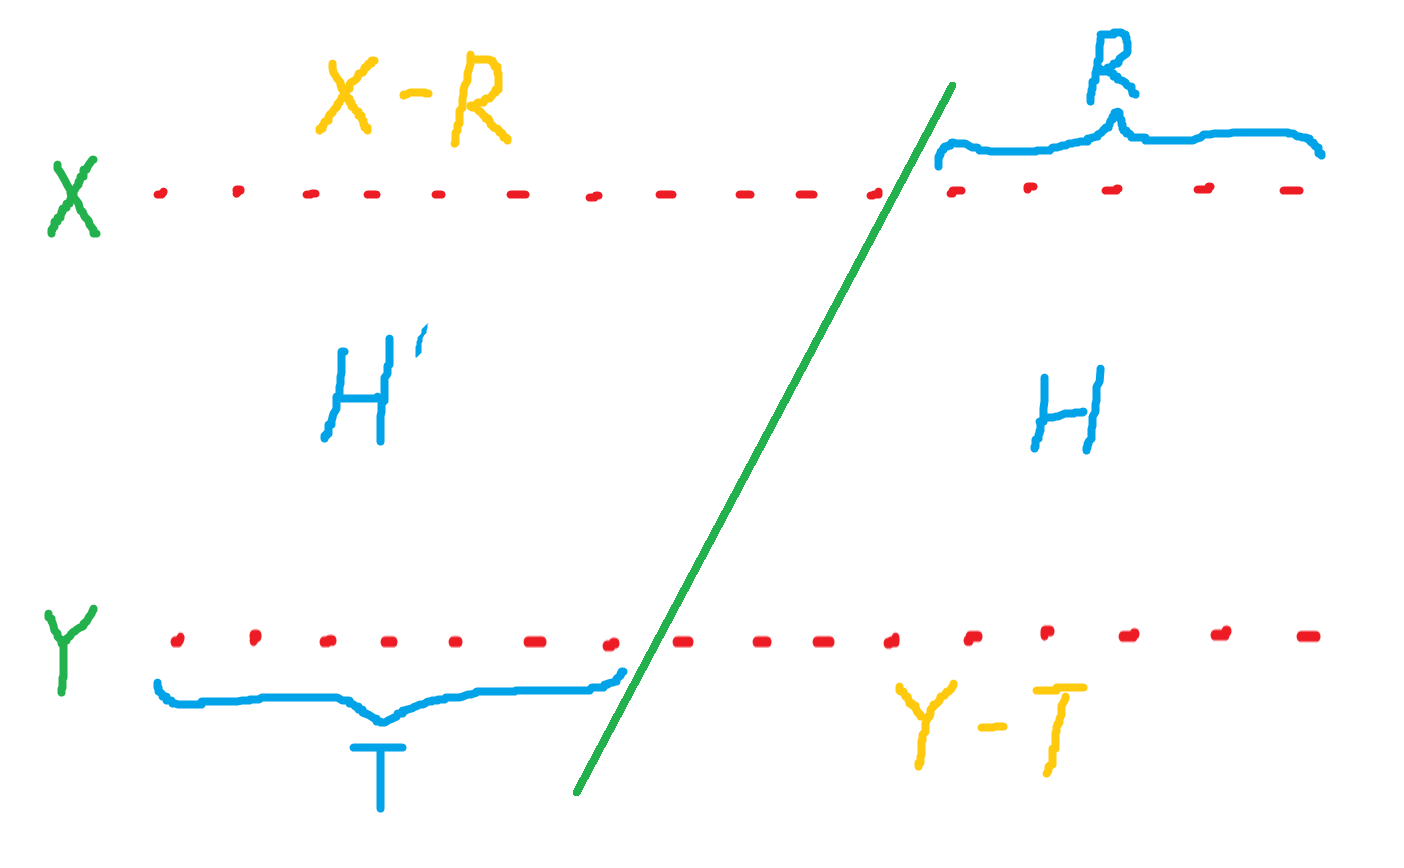
\includegraphics[width=0.5\textwidth]{img/proof_Konig_with_Hall.png}

            设二分图G的最小点覆盖为C$\alpha_0$,

            其中C在二分图子集X中的部分记为R,C在二分图子集Y中的部分记为T

            设R的任意子集为A,和A邻接的点集为p(A),

            其中在Y-T的部分记为$p_H(A)=p(A)\cap Y-T$,现欲证明$|p_H(A)|\ge|A|$

            假如$|p_H(A)|<|A|$,那么就可以得到点覆盖 $C'=C-A+p_H(A)$,

            使得$|C'|<|C|$,与C为最小点覆盖矛盾

            所以$|p_H(A)|\ge|A|$,即满足Hall定理的条件,

            所以存在匹配$M_R$,使得$|M_R|=|R|$

            同理可得存在匹配$M_T$,使得$|M_T|=|T|$

            所以图G中存在大小为$|M|=|R|+|T|=|C|$的匹配,

            由引理即可得$\beta_1(G)=\alpha_0(G)$,得证

            \vspace{1.5cm}


            \textbf{- 使用线性规划对偶定理来证明:}

            \vspace{0.3cm}

            \textbf{分数匹配的定义(Fractional matching)}

            图的分数匹配是对整数匹配的泛化,即允许每条边的匹配度为0到1之间的任意实数

            直观上来说,可以理解为把顶点分割为若干份,每份中的顶点都可以与另一顶点进行匹配

            \vspace{0.8cm}

            对于对于图G(V,E),如果存在一个实值函数$f:E\to R$,使得

            1. $\forall e\in E,f(e)\in[0,1]$

            2. $\forall v\in V,\sum_{e\ni v}f(e)\le1$

            那么称该实值函数f为图G的一个分数匹配

            对于任意图G(V,E),其最大分数匹配问题等价于:

            $$
                  \begin{aligned}
                        Maximize\quad     & 1_E\cdot x        \\
                        Subject\ to:\quad & x\ge0_E           \\
                                          & A_G\cdot x\le 1_V
                  \end{aligned}
            $$

            其中向量$x$是每条边的权重,故$1_E\cdot x$为图G的边权和,$Maximize$表示要尽可能多匹配边

            $x\ge0_E$指边权为非负数,$A_G$为图G的邻接矩阵,故$A_G\cdot x$为每个顶点的边权和

            $A_G\cdot x\le 1_V$表示每个顶点最多只能匹配一条完整边

            \vspace{0.8cm}

            对于任意图G(V,E),其最小分数点覆盖问题等价于:
            $$
                  \begin{aligned}
                        Minimize\quad     & 1_V\cdot y          \\
                        Subject\ to:\quad & y\ge0_V             \\
                                          & A_G^T\cdot y\ge 1_E
                  \end{aligned}
            $$
            向量$y$是每个顶点的权重,故$1_V\cdot y$为图G的顶点权和,$Minimize$表示要尽可能少点覆盖

            $y\ge0_V$指顶点权为非负数,$A_G^T$为图G的邻接矩阵的转置,故$A_G^T\cdot y$为每条边的顶点权和

            $A_G^T\cdot y\ge 1_E$表示每条边至少要被一个顶点覆盖

            由于最大分数匹配问题和最小点覆盖问题互为线性规划对偶,

            所以它们的最优解相等,即对于任意图,都有最大分数匹配等于最小分数点覆盖

            而对于二分图,两个问题的最优解都是整数解,

            所以对于二分图,有最大匹配等于最小点覆盖,得证



\end{enumerate}


\vspace{0.8cm}


\subsubsection{二分图最大基数匹配问题}

\textbf{Hopcroft–Karp算法}\cite{hopcroft1973n}

利用Dinic算法的思想,来实现分层搜索多条增广路

对于二分图G(X,Y),其算法实现如下

\vspace{0.5cm}

1. 将X中的未盖点作为$L(1)$,使用BFS算法构造 交错边层级图$G_L$

2. 如果在第k层找到位于Y的未盖点,那么$G_L$止步于第k层,并将第k层的所有未盖点记为F

3. 对于F中的每个Y未盖点,向上使用DFS搜索其对应的X未盖点,并将途经顶点标记为$used$

4. 如果向上找到了对应的X未盖点,那么就找到了一条增广路,删去这条增广路上途经的$used$顶点,保证这些顶点不会被下次搜索重复使用,重复步骤3和4直至F全部搜完

5. 重复步骤1到步骤4,直至不存在增广路为止

\vspace{1.5cm}

\textbf{- 定理}
Hopcroft–Karp算法的最差时间复杂度为$O(E\sqrt{V})$

由于每次迭代包含一次BFS和几次不重复的DFS,

所以每次迭代的时间复杂度为$O(E+E)=O(E)$

因此,对于刚开始的前$\sqrt{V}$次迭代,累计有时间复杂度为$O(E\sqrt{V})$

由于每次迭代至少会将最短增广路长度k增加1,

所以经过前$\sqrt{V}$次迭代后,此时的最短增广路长度至少为$\sqrt{V}$

不妨设此时的匹配为M,最终的最大匹配为M',

令$G'=M\oplus M'$,则$G'$中的连通分支皆为交错回路或者交错路

由于每条交错回路或交错路至少有$\sqrt{V}$条边,

则G'最多还有 $\frac{V}{\sqrt{V}}=\sqrt{V}$个连通分支,即M最多还有$\sqrt{V}$条增广路

故最多还需要$\sqrt{V}$次的增广迭代,再加上刚开始的前$\sqrt{V}$次迭代,故最多需要$2\sqrt{V}$次迭代,算法总共的时间复杂度为$O(E\sqrt{V})$,得证

\vspace{0.8cm}

\subsubsection{二分图最大权重匹配问题}

\textbf{Hungarian算法(Kuhn-Munkres算法)}\cite{munkres1957algorithms}

对于二分图G(S,T),定义实值函数 $y:(S\cup T)\to\mathbb{R}$

如果$\forall i\in S,j\in T$,都有$y(i)+y(j)\le c(i,j)$,则称y为G的一个潜在值函数(potential)

将$\sum_{v\in S\cup T}y(v)$,记为y的累加值,则可知任意完美匹配的值都至少会比y的累加值大

如果对于边$(i,j)$有$y(i)+y(j)=y(i,j)$,则称边$(i,j)$为y的紧致边(tight edges),

将由紧致边组成的图记为$G_y$,如果$G_y$中存在完美匹配,那么完美匹配的值就会等于y的值

\vspace{5cm}

对于匹配M,将S中的未盖点记为$R_S$,T中的未盖点记为$R_T$,

将从$R_S$出发的紧致交错路可达点记为$Z$

\vspace{0.5cm}

1. 如果$R_T\cap Z$不为空集,那么就存在一条从$R_S$到$R_T\cap Z$的增广路,将其加入匹配M中

2. 如果$R_T\cap Z$为空集,那么记$\Delta=\min\{c(i,j)-y(i)-y(j):i\in S\cap Z,j\in T-Z\}$

\vspace{0.5cm}

即$\Delta$为所有(左侧在交错路,右侧不在交错路的边)(的端点潜在值)(的最大可行增长)

对于左侧在紧致交错路中的顶点$s_z\in S\cup Z$,让其潜在值$f(s_z)+=\Delta$,

对于右侧在紧致交错路中的顶点$t_z\in T\cap Z$,让其潜在值$f(t_z\,)-=\Delta$

这样改变潜在值之后,$f(s_z)+=\Delta$ 只会影响下面两种边的端点值出现增加:

\vspace{0.2cm}

1. 对于左侧在$S\cup Z$,右侧在$T\cap Z$的边,

其两端点潜在值一增一减相互抵消,故$y'(i)+y'(j)=y(i)+y(j)$

\vspace{0.1cm}

2. 对于左侧在$S\cup Z$,右侧在$T-Z$的边,

其左端点潜在值增加值 为最大可行增长$\Delta$,不会导致$y(i)+y(j)> c(i,j)$

\vspace{0.5cm}

所以y仍然会是G的潜在值函数,并且经过迭代之后能够使得$G_y$中的紧致边数增加,

重复以上所有操作直到M成为完美匹配

\vspace{1.5cm}

\textbf{Hungarian算法有效性证明}

每次迭代后,会出现下面三种情况之一:

\vspace{0.15cm}

1. M已成为最大匹配

2. $R_T\cap Z$不为空集,则$G_y$存在增广路

3. $R_T\cap Z$为空集,则$G_y$存在紧致边的可行增长

\vspace{0.5cm}

由Berge定理可知,当M不是最大匹配时,图G中存在关于M的增广路P

1. 如果增广路P全部都在$G_y$中,那么通过对换即可得到更大的匹配

2. 如果增广路P不全在$G_y$,也就是说,尽管增广路P的偶数边(匹配边)根据M的定义都会在$G_y$中,但是它的奇数边(未匹配边)不一定会全部在$G_y$中

\vspace{0.5cm}

如果增广路P不全在$G_y$,不妨设此时增广路P的第一条松弛边为(u,v),

3. 如果v不在紧致交错路Z中,那么在计算$\Delta$时这条边(u,v)就会被计算在内,通过不断地可行增长能够使其最终成为$G_y$的一部分

4. 如果v会在紧致交错路Z中,那么存在一条紧致边(w,v),通过将增广路P中的(u,v)部分替换为(w,v)部分,仍然可以得到增广路P',并且P'的松弛边部分会比P的更短,对于P'再次重复3和4操作即可

\vspace{0.5cm}



\subsubsection{一般图最大基数匹配问题}

\textbf{Blossom算法}\cite{edmonds1965paths}

Blossom算法的核心是缩花与开花操作(Contractions and Blossoms)

\vspace{0.2cm}

\textbf{花朵的定义(blossom)}

对于任意图G(V,E)和匹配M,如果一个奇环有2k+1条边,并且其中有k条匹配边,那么称这个奇环为花朵(blossom)

\vspace{0.2cm}

花朵可以通过缩花,成为一个盖点$V_B$,图G经过缩花操作之后成为图G'

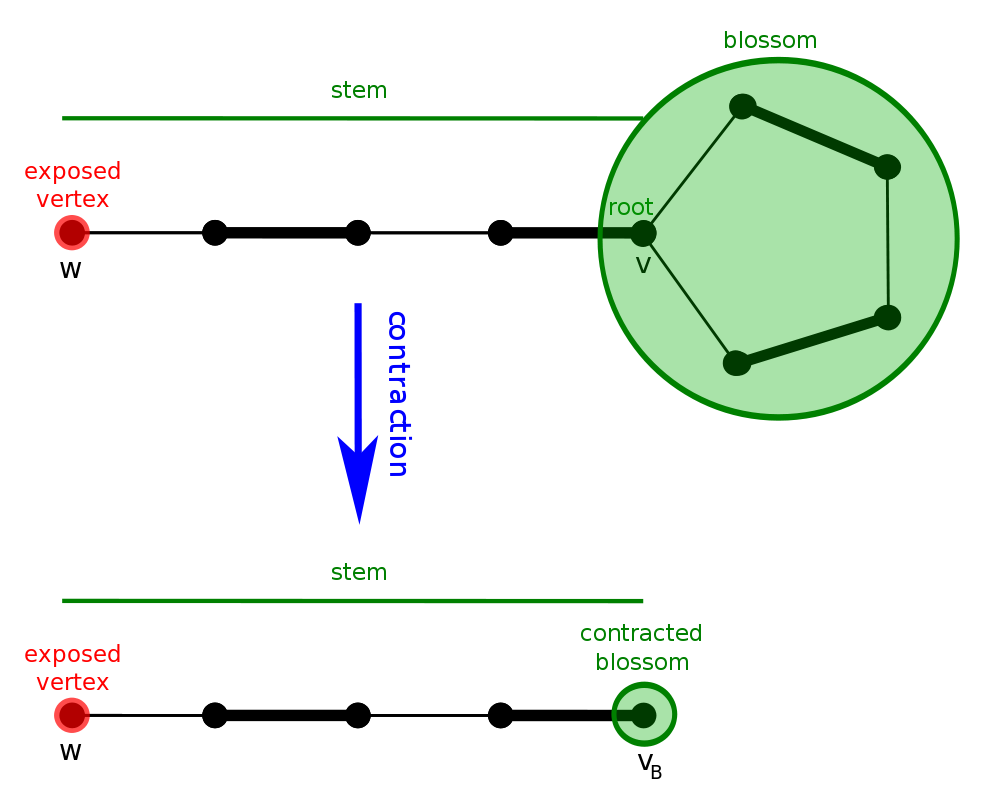
\includegraphics[width=0.55\textwidth]{img/1000px-Edmonds_blossom.svg.png}


\textbf{引理}
图G'有一条增广路P',当且仅当图G有一条增广路P

因为对于图G'中的增广路$P'=u\to v_B\to w$,可以通过开花将其替换为增广路$P=u\to(u'\to\cdots\to w')\to w$,其中$(u'\to\cdots\to w')$是经过花朵内部的交错路


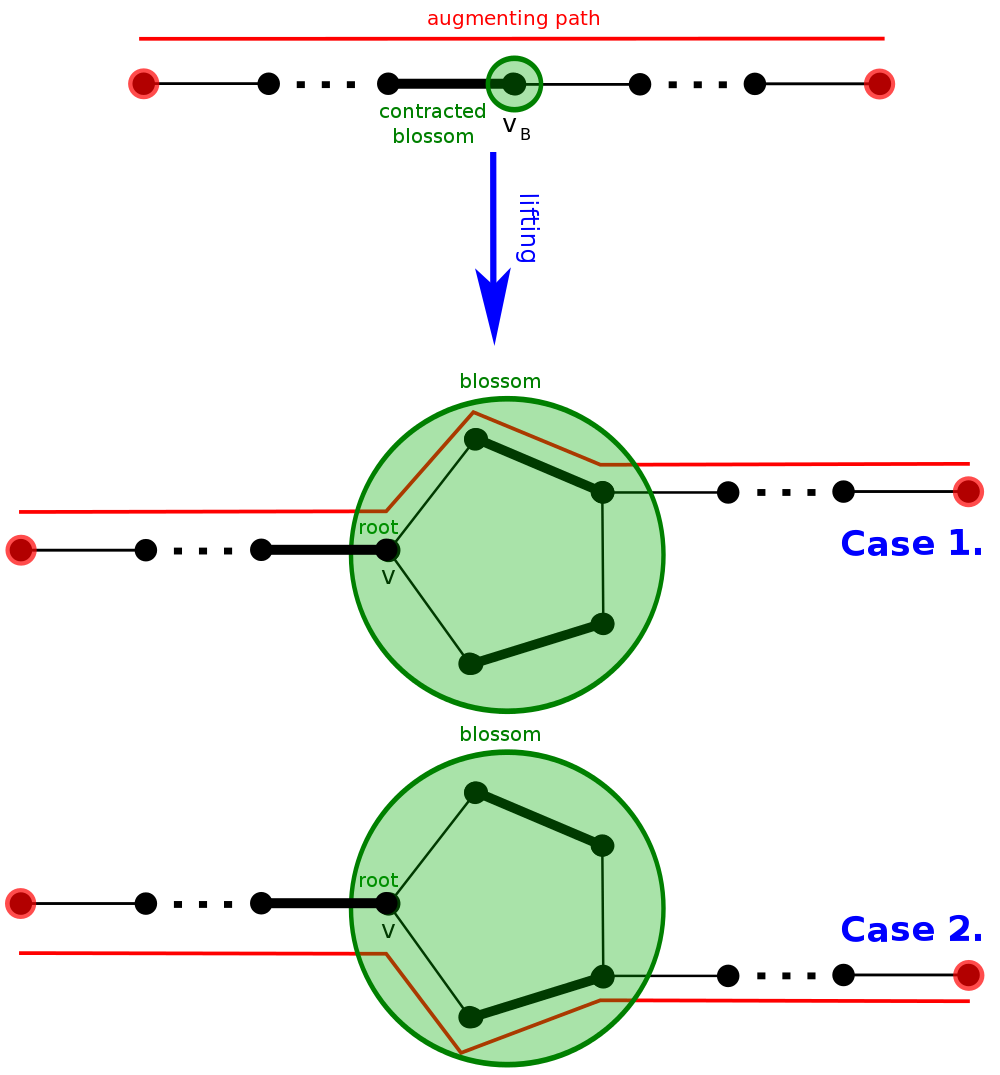
\includegraphics[width=0.6\textwidth]{img/1000px-Edmonds_lifting_path.svg.png}



\begin{algorithm}
      \caption{Blossom Algorithm}
      \begin{algorithmic}[1]
            \Procedure{find augmenting path}{$G,M$}
            \State \textbf{Input:} Graph G, matching M on G
            \State \textbf{Output:} augmenting path P in G or empty path if none found
            \State
            \State $F \gets$ empty forest
            \State unmark all vertices and edges in G, mark all edges of M
            \State
            \For{each exposed vertex v}
            \State create a singleton tree $\{v\}$ and add the tree to F
            \EndFor
            \State
            \While{an unmarked vertex v in F with distance(v, root(v)) even}
            \While{there exists an unmarked edge $e = \{v,w\}$}
            \If{w is not in F}
            \State // Add e and w's matched edge to expand F
            \State $x \gets$ vertex matched to w in M
            \State add edges $\{v,w\}$ and $\{w,x\}$ to the tree of v
            \ElsIf{w is in F}
            \If{distance(w, root(w)) is odd}

            \Else
            \If{root(v) $\neq$ root(w)}
            \State // Find an augmenting path in F $\cup$ \{e\}.
            \State $P \gets$ path $\{(root(v) \to ... \to v) \to (w \to ... \to root(w))\}$
            \State \textbf{return} P
            \ElsIf{root(v) == root(w)}
            \State // Look for the path in the contracted graph G'.
            \State $B \gets$ blossom formed by e and edges on the path v $\to$ w in T
            \State $G', M' \gets$ contract G and M by B
            \State $P' \gets$ find augmenting path(G', M')
            \State $P \gets$ lift P' to G
            \State \textbf{return} P
            \EndIf
            \EndIf
            \EndIf
            \State mark edge e
            \EndWhile
            \State mark vertex v
            \EndWhile
            \State \textbf{return} empty path
            \EndProcedure
      \end{algorithmic}
\end{algorithm}


\vspace{10.5cm}

\textbf{Blossom算法复杂度分析}

\vspace{0.1cm}

由于匹配M最多有$|V|/2$条边,最多要进行$|V|/2$次迭代

对于每次迭代过程中出现的两层循环嵌套,

外层嵌套的时间复杂度为$O(V)$,内层嵌套的时间复杂度为$O(E)$

所以每次迭代的时间复杂度为$O(EV)$,故Blossom算法的总时间复杂度为$O(EV^2)$


\subsubsection{一般图最大权重匹配问题}

综合使用Hungarian算法\cite{munkres1957algorithms}和Blossom算法\cite{edmonds1965paths}即可实现


\bibliographystyle{plain}
\bibliography{ref.bib}

\end{document}